\chapter{Boosting y árboles aditivos}\label{Chapter9} 
% chktex-file 8
% chktex-file 12
% chktex-file 13
% chktex-file 44


El boosting fue originalmente diseñado para problemas de clasificación, pero también puede extenderse de manera a regresión. La motivación para el boosting fue un procedimiento que combina las salidas de muchos clasificadores ``débiles'' para producir un ``comité'' poderoso. Desde esta perspectiva, el boosting guarda cierta similitud con el \textit{bagging} y otros enfoques basados en comités. Sin embargo, la conexión es, en el mejor de los casos, superficial, ya que el boosting es fundamentalmente diferente. \\

El algoritmo de boosting más popular es ``AdaBoost.M1''. Sea un problema de dos clases, con la variable de salida codificada como $Y \in \{-1, 1\}$. Dado un vector de variables predictoras $X$, un clasificador $G(X)$ produce una predicción que toma uno de los dos valores $\{-1, 1\}$. La tasa de error en la muestra de entrenamiento es
\begin{equation}
\frac{1}{N} \sum_{i=1}^{N} I(y_i \neq G(x_i))
\end{equation}

\noindent y la tasa de error esperada en futuras predicciones es $E_{XY} I(Y \neq G(X))$. \\

Un clasificador débil es aquel cuya tasa de error es ligeramente mejor que el clasificador aleatorio. El propósito del boosting es aplicar secuencialmente el algoritmo de clasificación débil a versiones modificadas de los datos, produciendo así una secuencia de clasificadores débiles $G_m(x)$, $m = 1,2,\dots,M$. \\

\begin{figure}[h]
\centering
\includegraphics[height=0.4\textheight]{fotos/67.png}
\caption{Esquema de AdaBoost. Los clasificadores se entrenan sobre versiones pesadas de los datos y se combinan para obtener la predicción final.}
\label{fig:67}
\end{figure}


Las predicciones de todos ellos se combinan mediante un voto mayoritario ponderado para producir la predicción final:
\begin{equation}
G(x) = \text{sign} \left( \sum_{m=1}^{M} \alpha_m G_m(x) \right)
\label{eq_boost:10.1}
\end{equation}

Aquí, $\alpha_1, \alpha_2, \dots, \alpha_M$ son calculadas por el algoritmo de boosting y ponderan la contribución de cada respectivo $G_m(x)$. Su efecto es dar mayor influencia a los clasificadores más precisos en la secuencia. La figura \ref{fig:67} muestra un esquema del procedimiento de AdaBoost. \\

Las modificaciones de los datos en cada paso de boosting consisten en aplicar pesos $w_1, w_2, \dots, w_N$ a cada una de las observaciones de entrenamiento $(x_i, y_i)$, $i = 1, 2, \dots, N$. Inicialmente, todos los pesos se establecen en $w_i = \frac{1}{N}$, de modo que el primer paso simplemente entrena el clasificador sobre los datos de la manera habitual. Para cada iteración sucesiva $m = 2, 3, \dots, M$, los pesos de observación son modificados individualmente y el algoritmo de clasificación se vuelve a aplicar a las observaciones ponderadas. En el paso $m$, aquellas observaciones que fueron mal clasificadas por el clasificador $G_{m-1}(x)$ inducido en el paso anterior tienen sus pesos incrementados, mientras que los pesos disminuyen para aquellas que fueron clasificadas correctamente. Así, a medida que las iteraciones progresan, las observaciones que son difíciles de clasificar correctamente reciben una influencia cada vez mayor. Cada clasificador sucesivo es forzado a concentrarse en aquellas observaciones de entrenamiento que fueron ignoradas por los clasificadores anteriores en la secuencia. \\

\begin{table}[h]
\centering
\begin{tabular}{l}
\toprule\toprule
\textbf{AdaBoost.M1} \\
\midrule\midrule
1. Inicializar los pesos de las observaciones $w_i = 1/N$, $i = 1, \dots, N$ \\
2. Para $m = 1$ hasta $M$: \\
\quad (a) Ajustar un clasificador débil $G_m(x)$ a los datos de entrenamiento usando los pesos $w_i$ \\
\quad (b) Calcular $\displaystyle \text{err}_m = \frac{\sum_{i=1}^{N} w_i I(y_i \neq G_m(x_i))}{\sum_{i=1}^{N} w_i}$ \\
\quad (c) Calcular $\displaystyle \alpha_m = \log \left((1 - \text{err}_m)/\text{err}_m \right)$ \\
\quad (d) Actualizar los pesos $w_i \leftarrow w_i \exp \left( \alpha_m I(y_i \neq G_m(x_i)) \right)$, $i = 1, \dots, N$ \\
3. Devolver $G(x) = \text{sign} \left( \sum_{m=1}^{M} \alpha_m G_m(x) \right)$ \\
\bottomrule\bottomrule
\end{tabular}
\caption{Algoritmo AdaBoost.M1}
\label{tb:10.1}
\end{table}


La tabla \ref{tb:10.1} muestra los detalles del algoritmo AdaBoost.M1. El clasificador actual $G_m(x)$ es inducido sobre las observaciones ponderadas en la línea 2a. La tasa de error ponderada resultante se computa en la línea 2b. La línea 2c calcula el peso $\alpha_m$ asignado a $G_m(x)$ para producir el clasificador final $G(x)$ (línea 3). Los pesos individuales de cada una de las observaciones son actualizados para la siguiente iteración en la línea 2d. Las observaciones mal clasificadas por $G_m(x)$ tienen sus pesos escalados por un factor $\exp(\alpha_m)$, incrementando su influencia relativa para inducir el siguiente clasificador $G_{m+1}(x)$ en la secuencia. \\

El algoritmo AdaBoost.M1 es conocido como “AdaBoost Discreto”, porque el clasificador base $G_m(x)$ retorna una etiqueta de clase discreta. Si el clasificador base, en cambio, retorna una predicción de valor real (por ejemplo, una probabilidad mapeada al intervalo $[-1, 1]$), AdaBoost puede ser modificado apropiadamente. \\



Generalmente, el clasificador débil es simplemente un ``stump'': un árbol de clasificación con dos nodos terminales. Aplicar este clasificador solo al conjunto de datos de entrenamiento da una tasa de error muy mala de prueba del 45.8\%, comparado con el 50\% para la adivinanza aleatoria. Sin embargo, a medida que las iteraciones de boosting progresan, la tasa de error disminuye constantemente, alcanzando el 5.8\% después de 400 iteraciones. Así, ``boostear'' este clasificador muy débil y simple reduce su tasa de error de predicción por casi un factor de cuatro. 

\section{Ajustes de \textit{boosting} y modelos aditivos}

El éxito del boosting realmente no es muy misterioso. La clave reside en la expresión (\ref{eq_boost:10.1}). El boosting es una forma de ajustar una expansión aditiva en un conjunto de funciones ``base'' elementales. Aquí, las funciones base son los clasificadores individuales $G_m(x) \in \{-1,1\}$. Más generalmente, las expansiones de funciones base toman la forma
\begin{equation}
f(x) = \sum_{m=1}^{M} \beta_m b(x; \gamma_m) 
\end{equation}

\noindent donde $\beta_m$, $m = 1,2,\dots,M$ son los coeficientes de expansión, y $b(x; \gamma) \in \mathbb{R}$ son usualmente funciones simples del argumento multivariable $x$, caracterizadas por un conjunto de parámetros $\gamma$. \\

Típicamente, estos modelos se ajustan minimizando una función de pérdida, como el error cuadrático o una función de pérdida basada en la verosimilitud, promediada sobre los datos de entrenamiento
\begin{equation}
\min_{\{\beta_m ,\gamma_m\}_1^M} \sum_{i=1}^{N} \frac{1}{N} L \left(y_i, \sum_{m=1}^{M} \beta_m b(x_i; \gamma_m)\right)
\label{eq_boost:10.4}
\end{equation}

Para muchas funciones de pérdida $L(y,f(x))$ y/o funciones base $b(x; \gamma)$, esto requiere técnicas de optimización numérica computacionalmente intensivas. Sin embargo, a menudo se puede encontrar una alternativa simple cuando es viable resolver rápidamente el subproblema de ajustar una sola función base,
\begin{equation}
\min_{\beta,\gamma} \sum_{i=1}^{N} L(y_i, \beta b(x_i; \gamma))
\end{equation}

\section{Modelado aditivo secuencial hacia delante}

El modelado secuencial hacia delante aproxima la solución a la ecuación (\ref{eq_boost:10.4}) añadiendo secuencialmente nuevas funciones base a la expansión sin ajustar los parámetros y coeficientes de aquellas que ya han sido añadidos. Esto se detalla en la tabla \ref{tb:10.2}. En cada iteración $m$, se resuelve para la función base óptima $b(x; \gamma_m)$ y el coeficiente correspondiente $\beta_m$ para añadir a la expansión actual $f_{m-1}(x)$. Esto produce $f_m(x)$, y el proceso se repite. Los términos añadidos previamente no se modifican. Para la pérdida de error cuadrático
\begin{equation}
L(y, f(x)) = (y - f(x))^2
\end{equation}

\noindent se tiene
\begin{align}
L(y_i, f_{m-1}(x_i) + \beta b(x_i; \gamma)) &= (y_i - f_{m-1}(x_i) - \beta b(x_i; \gamma))^2 \notag \\
& = (r_{im} - \beta b(x_i; \gamma))^2
\end{align}

\noindent donde $r_{im} = y_i - f_{m-1}(x_i)$ es simplemente el residuo del modelo actual en la observación $i$. Así, para la pérdida de error cuadrático, el término $\beta_m b(x; \gamma_m)$ que mejor se ajusta a los residuos actuales se añade a la expansión en cada paso. Esta idea es la base para el \textit{boosting} de regresión de mínimos cuadrados. Sin embargo, la pérdida de error cuadrático generalmente no es una buena elección para clasificación; de ahí la necesidad de considerar otros criterios de pérdida.

\begin{table}[h]
\centering
\begin{tabular}{l}
\toprule\toprule
\textbf{\textit{Forward Stagewise Additive Modeling}} \\
\midrule\midrule
1. Inicializar $f_0(x) = 0$ \\
2. Para $m = 1$ hasta $M$: \\
\quad (a) Calcular $\displaystyle (\beta_m, \gamma_m) = \underset{\beta, \gamma}{\text{argmin}} \sum_{i=1}^{N} L(y_i, f_{m-1}(x_i) + \beta b(x_i; \gamma))$ \\
\quad (b) Establecer $f_m(x) = f_{m-1}(x) + \beta_m b(x; \gamma_m)$ \\
\bottomrule\bottomrule
\end{tabular}
\caption{Algoritmo de modelado aditivo secuencial hacia delante}
\label{tb:10.2}
\end{table}

\section{Funciones de pérdida}

Se puede demostrar que AdaBoost.M1 es equivalente al modelado aditivo secuencial hacia delante utilizando la función de pérdida
\begin{equation}
L(y,f(x)) = \exp(-y f(x))
\end{equation}

Otro criterio de pérdida es el del logaritmo negativo de la verosimilitud binomial o desviación (también conocida como entropía cruzada), interpretando $f$ como la transformación \textit{logit}. Sea
\begin{equation}
p(x) = \Pr(Y = 1 | x) = \frac{e^{f(x)}}{e^{-f(x)} + e^{f(x)}} = \frac{1}{1 + e^{-2 f(x)}}
\end{equation}

\noindent y definiendo $Y' = (Y + 1)/2 \in \{0,1\}$. Entonces, la función de pérdida de log-verosimilitud binomial es
\begin{equation}
l(Y, p(x)) = Y' \log p(x) + (1 - Y') \log(1 - p(x))
\label{eq_boost:10.17}
\end{equation}

\noindent o de forma equivalente, la desviación es
\begin{equation}
-l(Y,f(x)) = \log\left(1 + e^{-2Y f(x)}\right)
\end{equation}

Dado que el máximo de la log-verosimilitud de población está en las probabilidades reales $p(x) = \Pr(Y = 1 | x)$, vemos a partir de (\ref{eq_boost:10.17}) que los minimizadores de población de la desviación $E_{Y|x}[-l(Y,f(x))]$ y $E_{Y|x}[e^{-Y f(x)}]$ son los mismos. Por lo tanto, usar cualquiera de los criterios conduce a la misma solución a nivel de población. \\

Con clasificación de $K$ clases, la respuesta $Y$ toma valores en el conjunto no ordenado $\mathcal{G} = \{\mathcal{G}_1, \dots, \mathcal{G}_K\}$. Ahora buscamos un clasificador $G(x)$ que tome valores en $\mathcal{G}$. Es suficiente conocer las probabilidades condicionales de clase $p_k(x) = \Pr(Y = \mathcal{G}_k \mid x)$, $k = 1,2,\dots,K$, pues entonces el clasificador de Bayes es
\begin{equation}
G(x) = \mathcal{G}_k \quad \text{donde} \quad k = \arg\max_\ell p_\ell(x)
\label{eq_boost:10.20}
\end{equation}

Sin embargo, en principio, no es necesario aprender los $p_k(x)$, sino simplemente cuál de ellos es el mayor. El modelo logístico se generaliza naturalmente a $K$ clases,
\begin{equation}
p_k(x) = \frac{e^{f_k(x)}}{\sum_{l=1}^{K} e^{f_l(x)}}
\label{eq_boost:10.21}
\end{equation}

\noindent lo que asegura que $0 \leq p_k(x) \leq 1$ y que suman uno. Nota que aquí tenemos $K$ funciones diferentes, una por clase. Existe una redundancia en las funciones $f_k(x)$, ya que añadir una función arbitraria $h(x)$ a cada una deja el modelo sin cambios. Tradicionalmente, una de ellas se establece a cero. Aquí preferimos mantener la simetría e imponer la restricción
\begin{equation}
\sum_{k=1}^{K} f_k(x) = 0.
\end{equation}

La desviación binomial se extiende naturalmente a la función de pérdida de desviación multinomial de $K$ clases:
\begin{align}
L(y, p(x)) &= -\sum_{k=1}^{K} I(y = \mathcal{G}_k) \log p_k(x) \notag \\ 
&= -\sum_{k=1}^{K} I(y = \mathcal{G}_k) f_k(x) + \log \sum_{\ell=1}^{K} e^{f_\ell(x)}
\label{eq_boost:10.22}
\end{align}

Como en el caso de dos clases, el criterio (\ref{eq_boost:10.22}) penaliza las predicciones incorrectas solo linealmente en su grado de incorrección. 

\begin{table}[h]
\centering
\begin{tabular}{lcccc}
\toprule\toprule
\textbf{Característica} & Redes neuronal & SVM & Árboles & KNN, kernels \\
\midrule\midrule
\makecell[l]{Manejo natural de datos \\ categóricos} & 

\begin{tikzpicture}
\fill[red] (0,0.433) -- (0.5,0.433) -- (0.25,0) -- cycle;
\end{tikzpicture} &

\begin{tikzpicture}
\fill[red] (0,0.433) -- (0.5,0.433) -- (0.25,0) -- cycle;
\end{tikzpicture} &
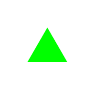
\begin{tikzpicture}
\fill[green] (0,0) -- (0.5,0) -- (0.25,0.433) -- cycle;
\end{tikzpicture} & 

\begin{tikzpicture}
\fill[red] (0,0.433) -- (0.5,0.433) -- (0.25,0) -- cycle;
\end{tikzpicture} \\ \midrule
Manejo de valores faltantes & 

\begin{tikzpicture}
\fill[red] (0,0.433) -- (0.5,0.433) -- (0.25,0) -- cycle;
\end{tikzpicture} &

\begin{tikzpicture}
\fill[red] (0,0.433) -- (0.5,0.433) -- (0.25,0) -- cycle;
\end{tikzpicture} &
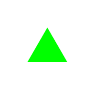
\begin{tikzpicture}
\fill[green] (0,0) -- (0.5,0) -- (0.25,0.433) -- cycle;
\end{tikzpicture} & 
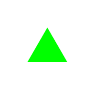
\begin{tikzpicture}
\fill[green] (0,0) -- (0.5,0) -- (0.25,0.433) -- cycle;
\end{tikzpicture} \\ \midrule
\makecell[l]{Robustez a \textit{outliers} en el \\ espacio de entrada} & 

\begin{tikzpicture}
\fill[red] (0,0.433) -- (0.5,0.433) -- (0.25,0) -- cycle;
\end{tikzpicture} &

\begin{tikzpicture}
\fill[red] (0,0.433) -- (0.5,0.433) -- (0.25,0) -- cycle;
\end{tikzpicture} &
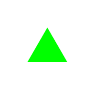
\begin{tikzpicture}
\fill[green] (0,0) -- (0.5,0) -- (0.25,0.433) -- cycle;
\end{tikzpicture} & 
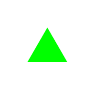
\begin{tikzpicture}
\fill[green] (0,0) -- (0.5,0) -- (0.25,0.433) -- cycle;
\end{tikzpicture} \\ \midrule
\makecell[l]{Insensibilidad a transformaciones \\ monótonas de las entradas} & 

\begin{tikzpicture}
\fill[red] (0,0.433) -- (0.5,0.433) -- (0.25,0) -- cycle;
\end{tikzpicture} &

\begin{tikzpicture}
\fill[red] (0,0.433) -- (0.5,0.433) -- (0.25,0) -- cycle;
\end{tikzpicture} &
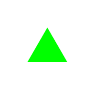
\begin{tikzpicture}
\fill[green] (0,0) -- (0.5,0) -- (0.25,0.433) -- cycle;
\end{tikzpicture} & 

\begin{tikzpicture}
\fill[red] (0,0.433) -- (0.5,0.433) -- (0.25,0) -- cycle;
\end{tikzpicture} \\ \midrule
\makecell[l]{Escalabilidad computacional \\ ($N$ grande)} & 

\begin{tikzpicture}
\fill[red] (0,0.433) -- (0.5,0.433) -- (0.25,0) -- cycle;
\end{tikzpicture} &

\begin{tikzpicture}
\fill[red] (0,0.433) -- (0.5,0.433) -- (0.25,0) -- cycle;
\end{tikzpicture} &
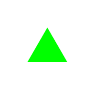
\begin{tikzpicture}
\fill[green] (0,0) -- (0.5,0) -- (0.25,0.433) -- cycle;
\end{tikzpicture} & 

\begin{tikzpicture}
\fill[red] (0,0.433) -- (0.5,0.433) -- (0.25,0) -- cycle;
\end{tikzpicture} \\ \midrule
\makecell[l]{Habilidad para manejar \\ entradas irrelevantes} & 

\begin{tikzpicture}
\fill[red] (0,0.433) -- (0.5,0.433) -- (0.25,0) -- cycle;
\end{tikzpicture} &

\begin{tikzpicture}
\fill[red] (0,0.433) -- (0.5,0.433) -- (0.25,0) -- cycle;
\end{tikzpicture} &
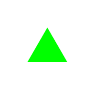
\begin{tikzpicture}
\fill[green] (0,0) -- (0.5,0) -- (0.25,0.433) -- cycle;
\end{tikzpicture} & 

\begin{tikzpicture}
\fill[red] (0,0.433) -- (0.5,0.433) -- (0.25,0) -- cycle;
\end{tikzpicture} \\ \midrule
\makecell[l]{Habilidad para extraer \\ combinaciones lineales \\ de las características} & 
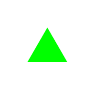
\begin{tikzpicture}
\fill[green] (0,0) -- (0.5,0) -- (0.25,0.433) -- cycle;
\end{tikzpicture} &
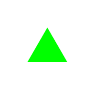
\begin{tikzpicture}
\fill[green] (0,0) -- (0.5,0) -- (0.25,0.433) -- cycle;
\end{tikzpicture} &

\begin{tikzpicture}
\fill[red] (0,0.433) -- (0.5,0.433) -- (0.25,0) -- cycle;
\end{tikzpicture} & 

\begin{tikzpicture}
\fill[orange] (0.25,0) -- (0.5,0.25) -- (0.25,0.5) -- (0,0.25) -- cycle;
\end{tikzpicture} \\ \midrule
Interpretabilidad & 

\begin{tikzpicture}
\fill[red] (0,0.433) -- (0.5,0.433) -- (0.25,0) -- cycle;
\end{tikzpicture} &

\begin{tikzpicture}
\fill[red] (0,0.433) -- (0.5,0.433) -- (0.25,0) -- cycle;
\end{tikzpicture} &

\begin{tikzpicture}
\fill[orange] (0.25,0) -- (0.5,0.25) -- (0.25,0.5) -- (0,0.25) -- cycle;
\end{tikzpicture} & 

\begin{tikzpicture}
\fill[red] (0,0.433) -- (0.5,0.433) -- (0.25,0) -- cycle;
\end{tikzpicture} \\ \midrule
Poder predictivo & 
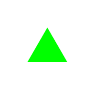
\begin{tikzpicture}
\fill[green] (0,0) -- (0.5,0) -- (0.25,0.433) -- cycle;
\end{tikzpicture} &
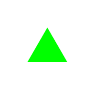
\begin{tikzpicture}
\fill[green] (0,0) -- (0.5,0) -- (0.25,0.433) -- cycle;
\end{tikzpicture} &

\begin{tikzpicture}
\fill[red] (0,0.433) -- (0.5,0.433) -- (0.25,0) -- cycle;
\end{tikzpicture} & 
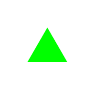
\begin{tikzpicture}
\fill[green] (0,0) -- (0.5,0) -- (0.25,0.433) -- cycle;
\end{tikzpicture} \\
\bottomrule\bottomrule
\end{tabular}
\caption{Características de los métodos de aprendizaje. Una forma de gestionar los valores faltantes en un árbol de decisión es la siguiente: si, por ejemplo, se llega a una división por la variable $X_1$, y a una muestra le falta el valor de $X_1$, se puede enviar la muestra por ambos caminos. La predicción final para esa muestra en clasificación la obtendremos promediando los vectores de probabilidad de todos los nodos hoja a los que llegue, mientras que en regresión será simplemente la media de los valores de las hojas a las que llegue.}
\label{tb:10.0}
\end{table}

\section{Árboles de \textit{boosting}}

Los árboles de regresión y clasificación se discuten en detalle en el capítulo \ref{Chapter6}. Dividen el espacio de todos los valores conjuntos de las variables predictoras en regiones disjuntas $R_j$, $j = 1, 2, \dots, J$, como se representa por los nodos terminales del árbol. Se asigna una constante $\gamma_j$ a cada una de dichas regiones y la regla predictiva es
\begin{equation}
x \in R_j \Rightarrow f(x) = \gamma_j
\end{equation}

\noindent Así, un árbol puede expresarse formalmente como
\begin{equation}
T(x; \Theta) = \sum_{j=1}^{J} \gamma_j I(x \in R_j)
\end{equation}

\noindent con parámetros $\Theta = \{R_j, \gamma_j\}_{j=1}^{J}$. $J$ generalmente se trata como un meta-parámetro. Los parámetros se encuentran minimizando el riesgo empírico
\begin{equation}
\hat{\Theta} = \arg\min_{\Theta} \sum_{j=1}^{J} \sum_{x_i \in R_j} L(y_i, \gamma_j)
\label{eq_boost:10.26}
\end{equation}

Este es un problema complicado de optimización combinatoria, y usualmente nos conformamos con soluciones subóptimas aproximadas. Es útil dividir el problema de optimización en dos partes:
\begin{itemize}
    \item \textbf{Encontrar $\gamma_j$ dado $R_j$:} Dado $R_j$, estimar $\gamma_j$ es típicamente trivial, y a menudo $\hat{\gamma}_j = \bar{y}_j$, es decir, la media de los $y_i$ que caen en la región $R_j$. Para la pérdida de clasificación errónea, $\hat{\gamma}_j$ es la clase modal de las observaciones que caen en la región $R_j$.
    \item \textbf{Encontrar $R_j$:} Esta es la parte difícil, para la cual se encuentran soluciones aproximadas. Nota también que encontrar $R_j$ implica estimar $\gamma_j$ también. Una estrategia típica es usar un algoritmo de particionamiento recursivo voraz de arriba hacia abajo para encontrar los $R_j$. Además, a veces es necesario aproximar (\ref{eq_boost:10.26}) mediante un criterio más suave y conveniente para optimizar los $R_j$:
    \begin{equation}
    \tilde{\Theta} = \arg\min_{\Theta} \sum_{i=1}^{N} \tilde{L}(y_i, T(x_i, \Theta))
    \label{eq_boost:10.27}
    \end{equation}
    
    Luego, dado los $R_j$, se puede estimar más precisamente los $\gamma_j$.
\end{itemize}

En el capítulo \ref{Chapter6} describimos esa estrategia para árboles de clasificación. El índice de Gini reemplazó la pérdida de clasificación errónea en el crecimiento del árbol (identificando los $R_j$). El modelo de árbol potenciado (``boosteado'') es una suma de árboles de este tipo,
\begin{equation}
f_M(x) = \sum_{m=1}^{M} T(x; \Theta_m)
\label{eq_boost:10.28}
\end{equation}

\noindent inducidos de manera secuencial hacia adelante (tabla \ref{tb:10.2}). En cada paso del procedimiento secuencial hacia delante, se debe resolver
\begin{equation}
\hat{\Theta}_m = \arg\min_{\Theta_m} \sum_{i=1}^{N} L(y_i, f_{m-1}(x_i) + T(x_i; \Theta_m))
\label{eq_boost:10.29}
\end{equation}

\noindent para el conjunto de regiones y constantes $\Theta_m = \{R_{jm}, \gamma_{jm}\}_{j=1}^{J_m}$ del siguiente árbol, dado el modelo actual $f_{m-1}(x)$. Dadas las regiones $R_{jm}$, encontrar los constantes óptimos $\gamma_{jm}$ en cada región es típicamente sencillo:
\begin{equation}
\hat{\gamma}_{jm} = \arg\min_{\gamma_{jm}} \sum_{x_i \in R_{jm}} L(y_i, f_{m-1}(x_i) + \gamma_{jm})
\label{eq_boost:10.30}
\end{equation}

Encontrar las regiones es difícil, y aún más difícil que para un solo árbol. Para algunos casos especiales, el problema se simplifica, como para mínimos cuadrados o clasificación binaria.

\section{Optimización numérica mediante \textit{Gradient Boosting}}

Por analogía con la optimización numérica, se pueden derivar algoritmos aproximados rápidos para resolver la ecuación (\ref{eq_boost:10.29}) con cualquier criterio de pérdida diferenciable. La pérdida al usar $f(x)$ para predecir $y$ en los datos de entrenamiento es
\begin{equation}
L(f) = \sum_{i=1}^{N} L(y_i, f(x_i))
\label{eq_boost:10.33}
\end{equation}

El objetivo es minimizar $L(f)$ con respecto a $f$, donde aquí $f(x)$ está restringida a ser una suma de árboles (\ref{eq_boost:10.28}). Ignorando esta restricción, minimizar (\ref{eq_boost:10.33}) puede verse como una optimización numérica
\begin{equation}
\hat{\mathbf{f}} = \arg\min_\mathbf{f} L(\mathbf{f})
\label{eq_boost:10.34}
\end{equation}

\noindent donde los ``parámetros'' $\mathbf{f} \in \mathbb{R}^N$ son los valores de la función de aproximación $f(x_i)$ en cada uno de los $N$ puntos de datos $x_i$:
\begin{equation}
f = \{f(x_1), f(x_2), \dots, f(x_N)\}^T
\end{equation}

Los procedimientos de optimización numérica resuelven (\ref{eq_boost:10.34}) como una suma de vectores componentes
\begin{equation}
\mathbf{f}_M = \sum_{m=0}^{M} \mathbf{h}_m, \quad \mathbf{h}_m \in \mathbb{R}^N,
\end{equation}

\noindent donde $\mathbf{f}_0 = \mathbf{h}_0$ es una estimación inicial, y cada $\mathbf{f}_m$ sucesivo se induce basado en el vector de parámetros actual $\mathbf{f}_{m-1}$, que es la suma de las actualizaciones inducidas previamente. Los métodos de optimización numérica difieren en sus prescripciones para calcular cada vector de incrementos $\mathbf{h}_m$ (``paso'').

\subsection{\textit{Steepest descent}}

El \textit{steepest descent} elige $\mathbf{h}_m = -\rho_m \mathbf{g}_m$, donde $\rho_m$ es un escalar y $\mathbf{g}_m \in \mathbb{R}^N$ es el gradiente de $L(\mathbf{f})$ evaluado en $\mathbf{f} = \mathbf{f}_{m-1}$. Los componentes del gradiente $\mathbf{g}_m$ son
\begin{equation}
g_{im} = \frac{\partial L(y_i, f(x_i))}{\partial f(x_i)} \bigg|_{f(x_i) = f_{m-1}(x_i)}
\label{eq_boost:10.35}
\end{equation}

\noindent La longitud del paso $\rho_m$ es la solución a
\begin{equation}
\rho_m = \arg\min_{\rho} L(\mathbf{f}_{m-1} - \rho \mathbf{g}_m)
\label{eq_boost:10.36}
\end{equation}

\noindent Luego, la solución actual se actualiza como
\begin{equation}
\mathbf{f}_m = \mathbf{f}_{m-1} - \rho_m \mathbf{g}_m
\end{equation}

\noindent y el proceso se repite en la siguiente iteración. El \textit{steepest descent} puede verse como una estrategia muy codiciosa, ya que $-\mathbf{g}_m$ es la dirección local en $\mathbb{R}^N$ para la cual $L(\mathbf{f})$ está decreciendo más rápidamente en $\mathbf{f} = \mathbf{f}_{m-1}$.

\subsection{\textit{Gradient Boosting}}

El boosting secuencial hacia delante (tabla \ref{tb:10.2}) también es una estrategia muy codiciosa. En cada paso, el árbol solución es aquel que reduce al máximo (\ref{eq_boost:10.29}), dado el modelo actual $f_{m-1}$ y sus ajustes $f_{m-1}(x_i)$. Así, las predicciones del árbol $T(x_i; \Theta_m)$ son análogas a los componentes del gradiente negativo (\ref{eq_boost:10.35}). La diferencia principal entre ellos es que los componentes del árbol $t_m = \{ T(x_1; \Theta_m), \dots, T(x_N; \Theta_m) \}^T$ no son independientes. Están restringidos a ser las predicciones de un árbol de decisión con $J_m$ nodos terminales, mientras que el gradiente negativo es la dirección de descenso máxima sin restricciones. \\

La solución a (\ref{eq_boost:10.30}) en el enfoque secuencial hacia delante es análoga a la búsqueda de línea (\ref{eq_boost:10.36}) en el \textit{steepest descent}. La diferencia es que (\ref{eq_boost:10.30}) realiza una búsqueda de línea separada para aquellos componentes de $t_m$ que corresponden a cada región terminal separada $\{ T(x_i; \Theta_m) \}_{x_i \in R_{jm}}$. \\

Si minimizar la pérdida en los datos de entrenamiento (\ref{eq_boost:10.33}) fuera el único objetivo, el \textit{steepest descent} sería la estrategia preferida. El gradiente (\ref{eq_boost:10.35}) es trivial de calcular para cualquier función de pérdida diferenciable $L(y,f(x))$, mientras que resolver (\ref{eq_boost:10.29}) es difícil para los criterios robustos discutidos anteriormente. Desafortunadamente, el gradiente (\ref{eq_boost:10.35}) está definido solo en los puntos de datos de entrenamiento $x_i$, mientras que el objetivo final es generalizar $f_M(x)$ a nuevos datos no representados en el conjunto de entrenamiento. \\

Una posible resolución a este dilema es inducir un árbol $T(x; \Theta_m)$ en la iteración $m$ cuyo predicciones $t_m$ sean lo más cercanas posible al gradiente negativo. Usando el error cuadrático para medir la cercanía, esto nos lleva a
\begin{equation}
\tilde{\Theta}_m = \arg\min_{\Theta_m} \sum_{i=1}^{N} \left( -g_{im} - T(x_i; \Theta) \right)^2
\label{eq_boost:10.37}
\end{equation}

Esto es, se ajusta el árbol $T$ a los valores del gradiente negativo (\ref{eq_boost:10.35}) por mínimos cuadrados. Existen algoritmos rápidos para la inducción de árboles de decisión por mínimos cuadrados. Aunque las regiones de solución $R_{jm}$ para (\ref{eq_boost:10.37}) no serán idénticas a las regiones $R_{jm}$ que resuelven (\ref{eq_boost:10.29}), generalmente son lo suficientemente similares como para cumplir el mismo propósito. En cualquier caso, el procedimiento de \textit{boosting} secuencial hacia delante y la inducción de árboles de decisión de arriba hacia abajo son, en sí mismos, procedimientos de aproximación. Después de construir el árbol (\ref{eq_boost:10.37}), las constantes correspondientes en cada región se dan por (\ref{eq_boost:10.30}). \\

Para la pérdida de error cuadrático, el gradiente negativo es simplemente el residuo ordinario $-g_{im} = y_i - f_{m-1}(x_i)$, de modo que (\ref{eq_boost:10.37}) por sí solo es equivalente al \textit{boosting} estándar de mínimos cuadrados. Con la pérdida de error absoluto, el gradiente negativo es el signo del residuo, por lo que en cada iteración (\ref{eq_boost:10.37}) ajusta el árbol al signo de los residuos actuales por mínimos cuadrados. \\

Para la clasificación, la función de pérdida es la desviación multinomial (\ref{eq_boost:10.22}), y se construyen $K$ árboles de mínimos cuadrados en cada iteración. Cada árbol $T_{km}$ se ajusta a su respectivo vector de gradiente negativo $g_{km}$,
\begin{align}
-g_{ikm} = \frac{\partial L(y_i, f_{1m}(x_i), \dots, f_{Km}(x_i))}{\partial f_{km}(x_i)} = I(y_i = G_k) - p_k(x_i)
\label{eq_boost:10.38}
\end{align}

\noindent con $p_k(x)$ dado por (\ref{eq_boost:10.21}). Aunque se construyen $K$ árboles separados en cada iteración, están relacionados a través de (\ref{eq_boost:10.21}). Para la clasificación binaria ($K=2$), solo se necesita un árbol.

\subsection{Implementación de \textit{Gradient Boosting}}

La tabla \ref{tb:10.3} presenta el algoritmo genérico de \textit{boosting} de árboles por gradiente para regresión. Se obtienen algoritmos específicos insertando diferentes criterios de pérdida $L(y, f(x))$. La primera línea del algoritmo inicializa con el modelo constante óptimo, que es simplemente un árbol con un único nodo terminal. Los componentes del gradiente negativo computados en la línea 2(a) se denominan residuos generalizados o pseudo residuos, $r$. \\

El algoritmo para clasificación es similar (tabla \ref{tb:10.4}). Las líneas 2(a)–(d) se repiten $K$ veces en cada iteración $m$, una vez para cada clase utilizando (\ref{eq_boost:10.38}). El resultado en la línea 3 son $K$ diferentes expansiones de árboles (acopladas) $f_k^M(x)$, $k = 1, 2, \dots, K$. Estos producen probabilidades mediante (\ref{eq_boost:10.21}) o realizan la clasificación como en (\ref{eq_boost:10.20}). \\

Dos parámetros básicos de ajuste son el número de iteraciones $M$ y los tamaños de cada uno de los árboles constituyentes $J_m$, $m = 1, 2, \dots, M$. La estrategia más simple para evitar es restringir que todos los árboles tengan el mismo tamaño, $J_m = J \ \forall m$. En cada iteración, se induce un árbol de regresión con $J$ nodos terminales. Así, $J$ se convierte en un meta-parámetro de todo el procedimiento de \textit{boosting}, que debe ajustarse para maximizar el rendimiento estimado para los datos disponibles.

\begin{table}[H]
\centering
\begin{tabular}{l}
\toprule\toprule
\textbf{\textit{Gradient Tree Boosting} (regresión)} \\
\midrule\midrule
1. Inicializar $f_0(x) = \arg\min_\gamma \sum_{i=1}^{N} L(y_i, \gamma)$ \\
2. Para $m = 1$ hasta $M$: \\
\quad (a) Para $i = 1, 2, \dots, N$, calcular $\displaystyle r_{im} = -\left[\frac{\partial L(y_i, f(x_i))}{\partial f(x_i)}\right]_{f(x_i) = f_{m-1}(x_i)}$ \\
\makecell[l]{\quad (b) Ajustar un árbol de regresión a los residuos generalizados $r_{im}$, dando regiones \\ \quad \quad \; $R_{jm}$, $j = 1, 2, \dots, J_m$} \\
\quad (c) Para $j = 1, 2, \dots, J_m$, calcular $\displaystyle \gamma_{jm} = \arg\min_\gamma \sum_{x_i \in R_{jm}} L(y_i, f_{m-1}(x_i) + \gamma)$ \\
\quad (d) Establecer $\displaystyle f_m(x) = f_{m-1}(x) + \sum_{j=1}^{J_m} \gamma_{jm} I(x \in R_{jm})$ \\
3. La salida será $\displaystyle \hat{f}(x) = f_M(x)$ \\
\bottomrule\bottomrule
\end{tabular}
\caption{Algoritmo de \textit{Gradient Tree Boosting} para regresión}
\label{tb:10.3}
\end{table}

\begin{table}[H]
\centering
\begin{tabular}{l}
\toprule\toprule
\textbf{\textit{Gradient Tree Boosting} (clasificación K clases)} \\
\midrule\midrule
1. Inicializar $f_{k0}(x) = 0$ para $k = 1, 2, \dots, K$ \\
2. Para $m = 1$ hasta $M$: \\
\quad (a) Fijar $\displaystyle p_k(x) = \frac{e^{f_{km-1}(x)}}{\sum_{l=1}^{K} e^{f_{lm-1}(x)}}$ para $k = 1, 2, \dots, K$ \\
\quad (b) Desde $k = 1$ hasta $K$: \\
\quad \quad (i) Calcular $\displaystyle r_{ikm} = y_{ik} - p_k(x_i)$, $i = 1, 2, \dots, N$ \\
\makecell[l]{\quad \quad (ii) Ajustar un árbol de regresión a los residuos generalizados $r_{ikm}$ (con $i = 1, \dots, N$), \\ \quad \quad \quad \; dando regiones $R_{jkm}$, $j = 1, 2, \dots, J_m$} \\
\quad \quad (iii) Calcular $\displaystyle \gamma_{jkm} = \frac{K - 1}{K} \frac{\sum_{x_i \in R_{jkm}} r_{ikm}}{\sum_{x_i \in R_{jkm}} |r_{ikm}|(1 - |r_{ikm}|)}$, $j = 1, \dots, J_m$ \\
\quad \quad (iv) Actualizar $\displaystyle f_{km}(x) = f_{k,m-1}(x) + \sum_{j=1}^{J_m} \gamma_{jkm} I(x \in R_{jkm})$ \\
3. La salida será $\displaystyle \hat{f}_k(x) = f_{kM}(x)$, $k = 1, \dots, K$. \\
\bottomrule\bottomrule
\end{tabular}
\caption{Algoritmo de \textit{Gradient Tree Boosting} para clasificación de $K$ clases}
\label{tb:10.4}
\end{table}

\section{Regularización}

Una forma conveniente de estimar $M^*$ es monitorear el riesgo de predicción en función de $M$ en una muestra de validación. El valor de $M$ que minimiza este riesgo se toma como una estimación de $M^*$. Esto es análogo a la estrategia de detención temprana que a menudo se usa con redes neuronales.

\subsection{Contracción}

Controlar el valor de $M$ no es la única posible estrategia de regularización. Al igual que en regresión Ridge y las redes neuronales, también se pueden emplear técnicas de contracción. La implementación más simple de contracción en el contexto del \textit{boosting} es escalar la contribución de cada árbol por un factor $0 < \nu < 1$ cuando se añade a la aproximación actual. Es decir, la línea 2(d) del algoritmo \ref{tb:10.3} se reemplaza por
\begin{equation}
f_m(x) = f_{m-1}(x) + \nu \cdot \sum_{j=1}^{J} \gamma_{jm} I(x \in R_{jm})
\label{eq_boost:10.41}
\end{equation}

El parámetro $\nu$ puede considerarse como el control de la tasa de aprendizaje del procedimiento de \textit{boosting}. Valores más pequeños de $\nu$ (más contracción) resultan en un mayor riesgo de entrenamiento para el mismo número de iteraciones $M$. Así, ambos $\nu$ y $M$ controlan el riesgo de predicción en los datos de entrenamiento. Sin embargo, estos parámetros no operan de manera independiente. Valores más pequeños de $\nu$ conducen a valores mayores de $M$ para el mismo riesgo de entrenamiento, de modo que existe una compensación entre ellos. \\

Empíricamente, se ha encontrado que valores más pequeños de $\nu$ favorecen un mejor error de prueba y requieren valores correspondientemente mayores de $M$. De hecho, la mejor estrategia parece ser establecer $\nu$ a valores muy pequeños $(\nu < 0.1)$ y luego elegir $M$ mediante detención temprana. El precio pagado por estas mejoras es computacional: valores más pequeños de $\nu$ generan valores mayores de $M$, y el cómputo es proporcional a este último.

\subsection{Submuestreo}

Con el \textit{boosting} por gradiente estocástico, en cada iteración se muestrea una fracción $\eta$ de las observaciones de entrenamiento (sin reemplazo), y se crece el siguiente árbol utilizando esa submuestra. El resto del algoritmo es idéntico. Un valor típico para $\eta$ puede ser $1/2$, aunque para grandes $N$, $\eta$ puede ser significativamente menor. La desventaja es que ahora tenemos cuatro parámetros a establecer: $J$, $M$, $\nu$ y $\eta$. Normalmente, algunas exploraciones iniciales determinan valores adecuados para $J$, $\nu$ y $\eta$, dejando $M$ como el parámetro principal a determinar por validación cruzada.

\section{Interpretación}

Los árboles de decisión individuales son altamente interpretables. El modelo completo puede ser completamente representado por un gráfico bidimensional simple (árbol binario) que es fácilmente visualizable. Las combinaciones lineales de árboles (\ref{eq_boost:10.28}) pierden esta característica importante y, por lo tanto, deben interpretarse de una manera diferente.

\subsubsection{Importancia relativa de las variables predictoras}

Las variables predictoras de entrada rara vez son igualmente relevantes. A menudo, solo unas pocas de ellas tienen una influencia sustancial en la respuesta; la gran mayoría son irrelevantes y podrían no haber sido incluidas. Por esto, es útil aprender la importancia relativa o contribución de cada variable de entrada en la predicción de la respuesta. Para un solo árbol de decisión $T$, se propone
\begin{equation}
\mathcal{I}_\ell^2 (T) = \sum_{t=1}^{J-1} \hat{i}_t^2 I(v(t) = \ell)
\label{eq_boost:10.42}
\end{equation}

\noindent como una medida de relevancia para cada variable predictora $X_\ell$. La suma es sobre los $J - 1$ nodos internos del árbol. En cada uno de dichos nodos $t$, se usa una de las variables de entrada $X_{v(t)}$ para dividir la región asociada con ese nodo en dos subregiones; dentro de cada una, se ajusta una constante separada a los valores de respuesta. La variable particular elegida es aquella que da la mejora máxima estimada $\hat{i}_t^2$ en el riesgo de error cuadrático sobre la de un ajuste constante sobre toda la región. La importancia relativa al cuadrado de la variable $X_\ell$ es la suma de tales mejoras al cuadrado sobre todos los nodos internos para los cuales fue elegida como la variable de división. \\

Esta medida de importancia se generaliza fácilmente a expansiones aditivas de árboles (\ref{eq_boost:10.28}); simplemente se promedia sobre los árboles
\begin{equation}
\mathcal{I}_\ell^2 = \frac{1}{M} \sum_{m=1}^{M} \mathcal{I}_\ell^2(T_m)
\label{eq_boost:10.43}
\end{equation}

Debido al efecto estabilizador del promedio, esta medida resulta ser más fiable que su contraparte (\ref{eq_boost:10.42}) para un solo árbol.